% senior_thesis-proposal.tex
% CMPSC 580, Spring 2016
%
%
% This document provides a sample senior thesis proposal template for use
% by students in Allegheny's CS and Applied Computing programs.
%
%   *******************************************************************
%   * LOOK FOR BLOCK COMMENTS SUCH AS THIS ONE FOR AN EXPLANATION OF  *
%   * THIS DOCUMENT AND HOW TO MODIFY IT FOR YOUR OWN PROPOSAL!       *
%   *                                                                 *
%   * ANY LINE BEGINNING WITH A "%" IS A LATEX COMMENT AND IS IGNORED *
%   * BY THE LATEX PROCESSOR. YOU ARE ENCOURAGED TO COMMENT YOUR OWN  *
%   * LATEX CODE.                                                     *
%   *******************************************************************

%   ********************************************************************
%   * THE FIRST SECTION OF THE LATEX FILE IS THE "PREAMBLE." IT        *
%   * INSTRUCTS LATEX TO IMPORT SPECIAL PACKAGES FOR THINGS LIKE       *
%   * INCLUDING FIGURES, DOUBLE-SPACING, COLORED TEXT, ETC.            *
%   * DEPENDING ON YOUR NEEDS, YOU MAY FIND IT NECESSARY TO USE PACK-  *
%   * AGES THAT ARE NOT INCLUDED IN THIS TEMPLATE. SIMPLY IMITATE THE  *
%   * "\usepackage{...}" COMMANDS SHOWN BELOW.                         *
%   ********************************************************************

%   ********************************************************************
%   * BEGINNING OF PREAMBLE:                                           *
%   ********************************************************************
\documentclass[11pt]{article}

\usepackage[T1]{fontenc}
\usepackage{mathptmx}
\topmargin 0.0in
\setlength{\textwidth} {420pt}
\setlength{\textheight} {620pt} 
\setlength{\oddsidemargin} {20pt}
\setlength{\marginparwidth} {72in}

%   ********************************************************************
%   * Many of the commands below were simply copied over from an older *
%   * version of the proposal template; you can just leave them as     *
%   * they are (or you can delve into the TeX/LaTeX documentation      *
%   * and figure out what they do). Otherwise, jump ahead to the next  *
%   * block of comments, where you will enter title, abstract, etc.    *
%   ********************************************************************

\usepackage{fancyhdr} 
\usepackage{url}
\usepackage{graphicx}

% set it so that subsubsections have numbers and they
% are displayed in the TOC (maybe hard to read, might want to disable)

\setcounter{secnumdepth}{3}
\setcounter{tocdepth}{3}

% define widow protection

\def\widow#1{\vskip #1\vbadness10000\penalty-200\vskip-#1}

\clubpenalty=10000  % Don't allow orphans
\widowpenalty=10000 % Don't allow widows

% this should give me the ability to use some math symbols that 
% were available by default in standard latex (i.e. \Box)

\usepackage{latexsym}

% define a little section heading that doesn't go with any number

\def\littlesection#1{
\widow{2cm}
\vskip 0.5cm
\noindent{\bf #1}
\vskip 0.0001cm 
}

\pagestyle{fancyplain}

\newcommand{\tstamp}{\today}   
\renewcommand{\sectionmark}[1]{\markright{#1}}
\lhead[\Section \thesection]            {\fancyplain{}{\rightmark}}
\chead[\fancyplain{}{}]                 {\fancyplain{}{}}
\rhead[\fancyplain{}{\rightmark}]       {\fancyplain{}{\thepage}}
\cfoot[\fancyplain{\thepage}{}]         {\fancyplain{\thepage}{}}

\newlength{\myVSpace}% the height of the box
\setlength{\myVSpace}{1ex}% the default, 
\newcommand\xstrut{\raisebox{-.5\myVSpace}% symmetric behaviour, 
  {\rule{0pt}{\myVSpace}}%
}

% leave things with no spacing extra spacing in the final version of the paper
\renewcommand{\baselinestretch}{1.0}    % must go before the begin of doc

% suppress the use of indentation for a paragraph

\setlength{\parindent}{0.0in}
\setlength{\parskip}{0.1in}

\begin{document}


% handle widows appropriately
\def\widow#1{\vskip #1\vbadness10000\penalty-200\vskip-#1}

% build the title section

\makeatletter

\def\maketitle{%
  %\null
  \thispagestyle{empty}%
  %\vfill
  \begin{center}%\leavevmode
    %\normalfont
    {\Huge \@title\par}%
    %\hrulefill\par
    {\normalsize \@author\par}%
    \vskip .4in
%    {\Large \@date\par}%
  \end{center}%
  %\vfill
  %\null
  %\cleardoublepage

  }

\makeatother

%   ********************************************************************
%   * Here is the first place where you need to begin customizing:     *
%   * Enter you name, the title of your proposal, etc., in the places  *
%   * indicated by the comment "% CHANGE!".                            *
%   ********************************************************************

\vspace*{-1.1in}
\title{Title of Your Senior Thesis Proposal}  % CHANGE!

% build the author section
\author{
        Your Full Name\\  % CHANGE!
        Department of Computer Science\\
        Allegheny College \\
        {\tt youremail@allegheny.edu}  \\  % CHANGE!
        \url{http://www.cs.allegheny.edu/~yourwebsite/} \\  % CHANGE OR DELETE!
        \vspace*{.1in} \today \\ \vspace*{.1in}
}

\maketitle       % use the default title stuff

% Default "abstract" environment is too small; customize one instead:
\begin{center}
\large\bf Abstract
\vspace{-1em}  % Reduce space between header and the abstract
\end{center}

%   ********************************************************************
%   * Here is the second place where you need to customize:            *
%   * enter your abstract in the "quote" environment:                 *
%   ********************************************************************

\begin{quote}
Provide a concise summary of your proposed research. Remember that
the abstract is {\it not} an introduction, it is a {\it summary} of the
entire document. It makes sense to wait to write the abstract until the
rest of the document has been written.
\end{quote}

%\vspace*{-.4in}
\section{Introduction}
\label{sec:introduction}
\vspace*{-.1in}

%   ********************************************************************
%   * Enter the text of your introductory section here.                *
%   ********************************************************************

Provide an intuitive motivation for and introduction to your proposed
senior thesis research.  Whenever possible, you should use one or more
concrete examples and technical diagrams.

\vspace*{-.1in}
\section{Related Work}
\label{sec:relatedwork}
\vspace*{-.1in}

%   ********************************************************************
%   * Enter the text of your related work section here.                *
%   ********************************************************************

Summarize the previously published papers and books that are related
to your proposed research.  Whenever possible, you should compare and
constrast your approach with the ones that have been discussed in the
past.  As you describe your papers, please make sure that you cite
them properly \cite{conrad-gecco-selection-study}.

\vspace*{-.2in}
\section{Method of Approach}
\label{sec:method}
\vspace*{-.1in}

%   ********************************************************************
%   * Enter the text of your method of approach section here.          *
%   ********************************************************************

Use technical diagrams, equations, algorithms, and paragraphs of text
to describe the research that you intend to complete. See the \LaTeX\ source
file for the proposal to learn how Figure \ref{intro-fig1} and Table 
\ref{intro-tab1} were included. Be sure to number all figures and tables and to
explicitly refer to them in your text.

\begin{figure}[htbp]
\centering
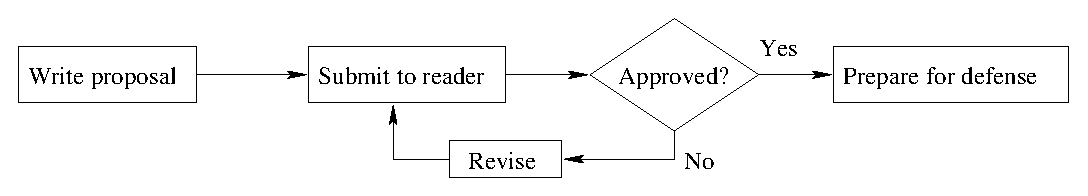
\includegraphics[width=5in]{flow}
\caption{Flow graph for proposal-writing}
\label{intro-fig1}
\end{figure}

\begin{table}[htbp]
\centering
\begin{tabular}{|c||c|c|}
\hline
\bf Task & \bf Begin Date & \bf End Date\\\hline\hline
First draft & Now & 20 Sept\\\hline
Second draft & 20 Sept & 27 Sept\\\hline
Third draft & 27 Sept & 4 Oct\\\hline
Fourth draft & 4 Oct & 11 Oct\\\hline
Fifth draft & 11 Oct & 18 Oct\\\hline
\end{tabular}
\caption{Proposed work schedule}
\label{intro-tab1}
\end{table}

\vspace*{-.2in}
\section{Evaluation Strategy}
\label{sec:evaluate}
\vspace*{-.1in}

%   ********************************************************************
%   * Enter the text of your evaluation strategy section here.         *
%   ********************************************************************

Explain what steps you will take to evaluate your proposed method.  If
you intend to conduct experiments, then you must clearly define your
evaluation metrics.

\vspace*{-.1in}
\section{Research Schedule}
\label{sec:schedule}
\vspace*{-.1in}

Identify the main phases and tasks of your research project and set
deadlines for when you will be able to complete each of these items.

\vspace*{-.1in}
\section{Conclusion}
\label{sec:conclusion}
\vspace*{-.1in}

%   ********************************************************************
%   * Enter the text of your concluding section section here.          *
%   ********************************************************************

Provide a summary of your proposed research and suggest the impact
that it may have on the discipline of computer science.  If possible,
you may also suggest some areas for future research \cite{jia2011analysis}.

\bibliographystyle{plain}
\bibliography{senior_thesis_proposal}

\end{document}

